\section{Assignment 13}

\subsection{Implement the admittance control in the operational space}

\begin{figure}[H]
\centering
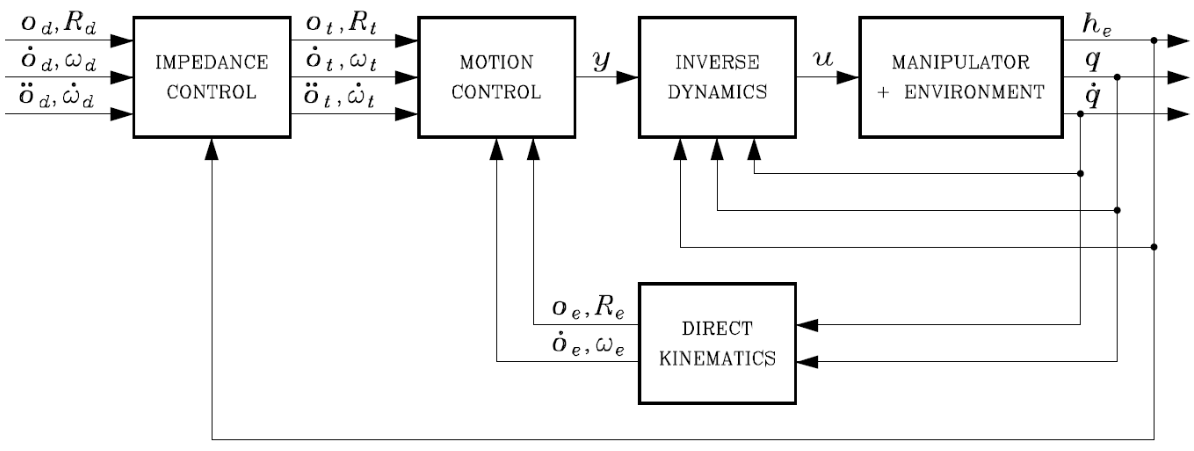
\includegraphics[keepaspectratio,width=.5\textwidth]{admittance_arch}
\caption{Admittance control in operational space architecture}
\end{figure}

The relationship between the external interaction force $h_e^d$ and the operational space error $\tilde z$ is defined through an admittance:

\begin{equation*}
M_t\ddot{\tilde z}+K_D\dot{\tilde z}+K_P\tilde z = h_e^d
\end{equation*}

The operational space error is between the desired frame and a compliant frame, introduce to force a compliant behaviour of the end-effector. The manipulator then always follows the compliant trajectory, which is equal to the desired one only in absence of external disturbances.

The architecture is modelled in SIMULINK as follows:

\begin{figure}[H]
\centering
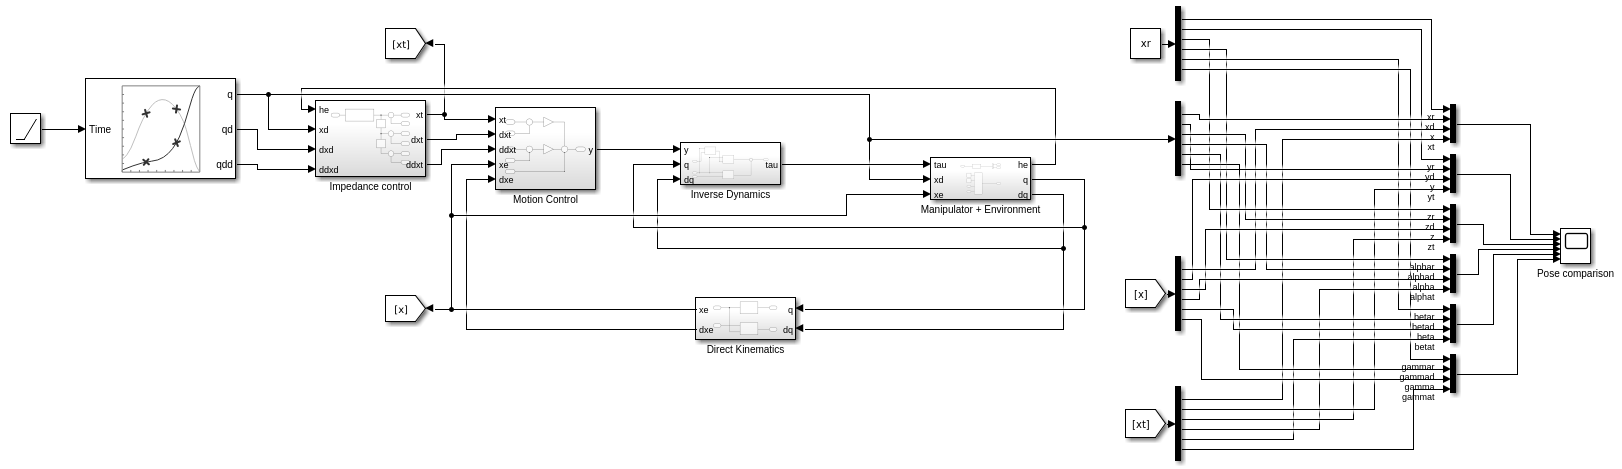
\includegraphics[keepaspectratio,width=\textwidth]{admittance_sim}
\caption{Admittance control in operational space SIMULINK model}
\end{figure}

To test the architecture, the manipulator was moved to $x_0=k(\begin{bmatrix}
0&-0.3&0
\end{bmatrix})$, with a desired position of $x_d=k(\begin{bmatrix}
0&-0.25&0
\end{bmatrix})$ and the environment placed at $x_e=k(\begin{bmatrix}
0&-0.2&0
\end{bmatrix})$. This was done to simplify the architecture, allowing for contact only in the $y$ direction. The mechanical impedance was defined with $M_t=\begin{bmatrix}
1 & 1 & 1 & 1 & 1 & 1
\end{bmatrix}$, $K_{Dt}=\begin{bmatrix}
1 & 10 & 1 & 1 & 1 & 1
\end{bmatrix}$ and $K_{Pt}=\begin{bmatrix}
1 & 20 & 1 & 1 & 1 & 1
\end{bmatrix}$ , while the control law is defined by $K_D=\begin{bmatrix}
10 & 10 & 10 & 10 & 10 & 10
\end{bmatrix}$ and $K_P=\begin{bmatrix}
50 & 50 & 50 & 50 & 50 & 50
\end{bmatrix}$.


\newpage

\begin{figure}[H]
\centering
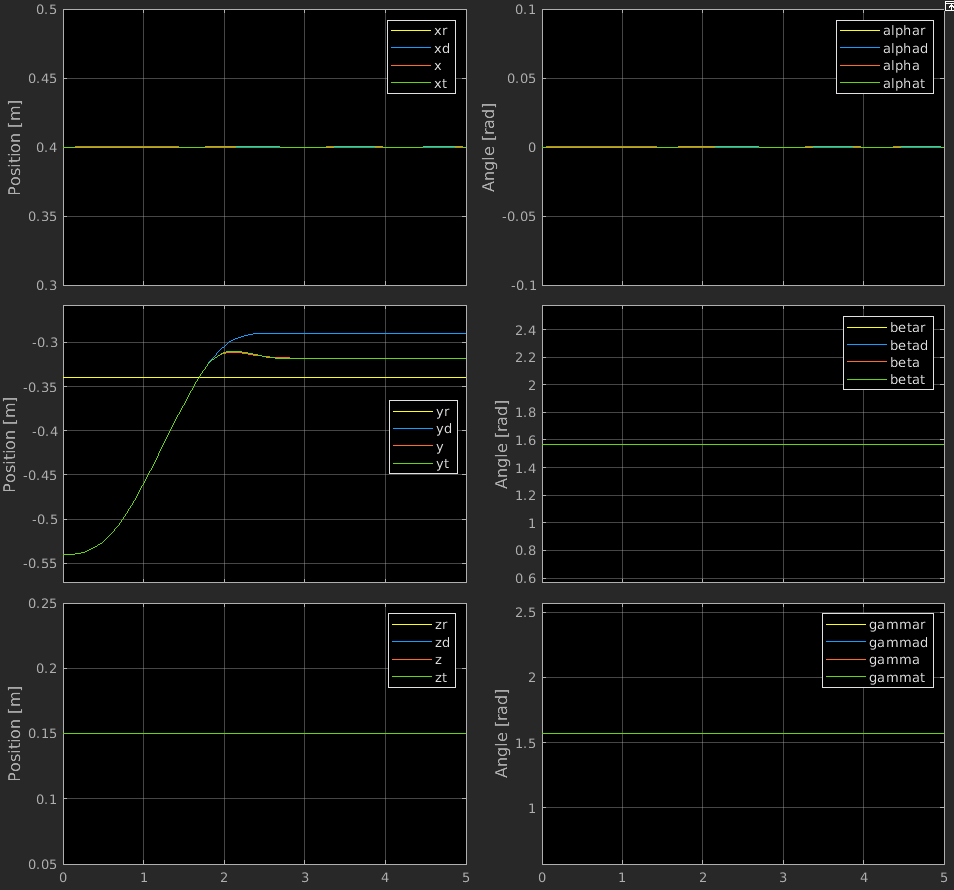
\includegraphics[keepaspectratio,width=\textwidth]{admittance_1}
\caption{Admittance control}
\end{figure}